\newcommand{\xbr}{\left(x\right)}
\newcommand{\br}[1]{\left(#1\right)}


\chapter{The model}

The system being under consideration consists of two 1D s-type superconducting wires connected with a tunnel junction. There is a strong spin-orbit coupling assumed to be present and external magnetic field is applied in the direction perpendicular to the wire. The Hamiltonianm of the bulk of each wire, written in the Bogoliubov-de Gennes formalism, is similar to the ones presented in \cite{Oreg_2010} and \cite{Lutchyn_2010}:

\begin{gather}
	\mathcal{H}
	=
	\int dy ~
	\Psi^\dagger
	\br{y}
	H
	\Psi
	\br{y}
	\
	~~~~
	\Psi
%	\left(x\right)
	=
	\begin{pmatrix}
		\psi_\uparrow
		\\
		\psi_\downarrow
		\\
		\psi_\downarrow^\dagger
		\\
		-\psi_\uparrow^\dagger
	\end{pmatrix}
	\\
	\label{bulk_Hamiltonian}
	H
	=
	\br{
		\frac{p^2}{2m}
		-\mu_0
	}\tau_z
	+
	u p \sigma_z \tau_z
	+
	B\sigma_x	
	+
	\Delta\tau_\phi
\end{gather}

Here $ \sigma_i $ and $ \tau_i $ are Pauli matrices in spin and particle-hole subspaces respectfully, $ \tau_\phi = \tau_x \cos\phi - \tau_y \sin\phi$, with $ \phi $ being a superconducting phase. $ \mu_0 $ is a chemical potential, $ B $ is an external magnetic field, $ \Delta $ is the module of superconducting order parameter and $ u $ is spin-orbit coupling constant with the dimension of velocity. The wire is being aligned along the y-axis, while the direction of the magnetic field coincides with x-axis. Note, that only one component of spin-orbit is nonzero due to 1D nature of the problem.

The tunnel junction is introduced  by applying an external electrical field. It's potential profile $U\br{y}  $ is presented at figure \ref{fig:chemandextpotentials}(a). Inside each wire the potential is assumed to be homogeneous, thought it's value can be different to the right and to the left of the junction. The junction itself is modeled by a sharp pike of the potential.
 
To take this into account it's necessary to include an additional term $ U \br{y}\tau_z $ in (\ref{bulk_Hamiltonian}). However this term can be combined with the second term of  by (\ref{bulk_Hamiltonian}) by introducing an effective chemical potential $ \mu \br{y} = \mu_0 - U\br{y}  $ (see figure \ref{fig:chemandextpotentials}(b)). From now on all presence of  the external field will be hidden in $ \mu\br{y} $.

The superconducting phase $ \phi $ in left and right wires, $ \phi_L $ and $ \phi_R $, can also be different. The phase inside the barrier is assumed to be a continuous monotonous function going from $ \phi_L $ to $ \phi_R $. The exact shape of that function is not important, as $ \mu\br{y} \gg \Delta$ inside the   
barrier.



\begin{figure}[H]
	\centering
	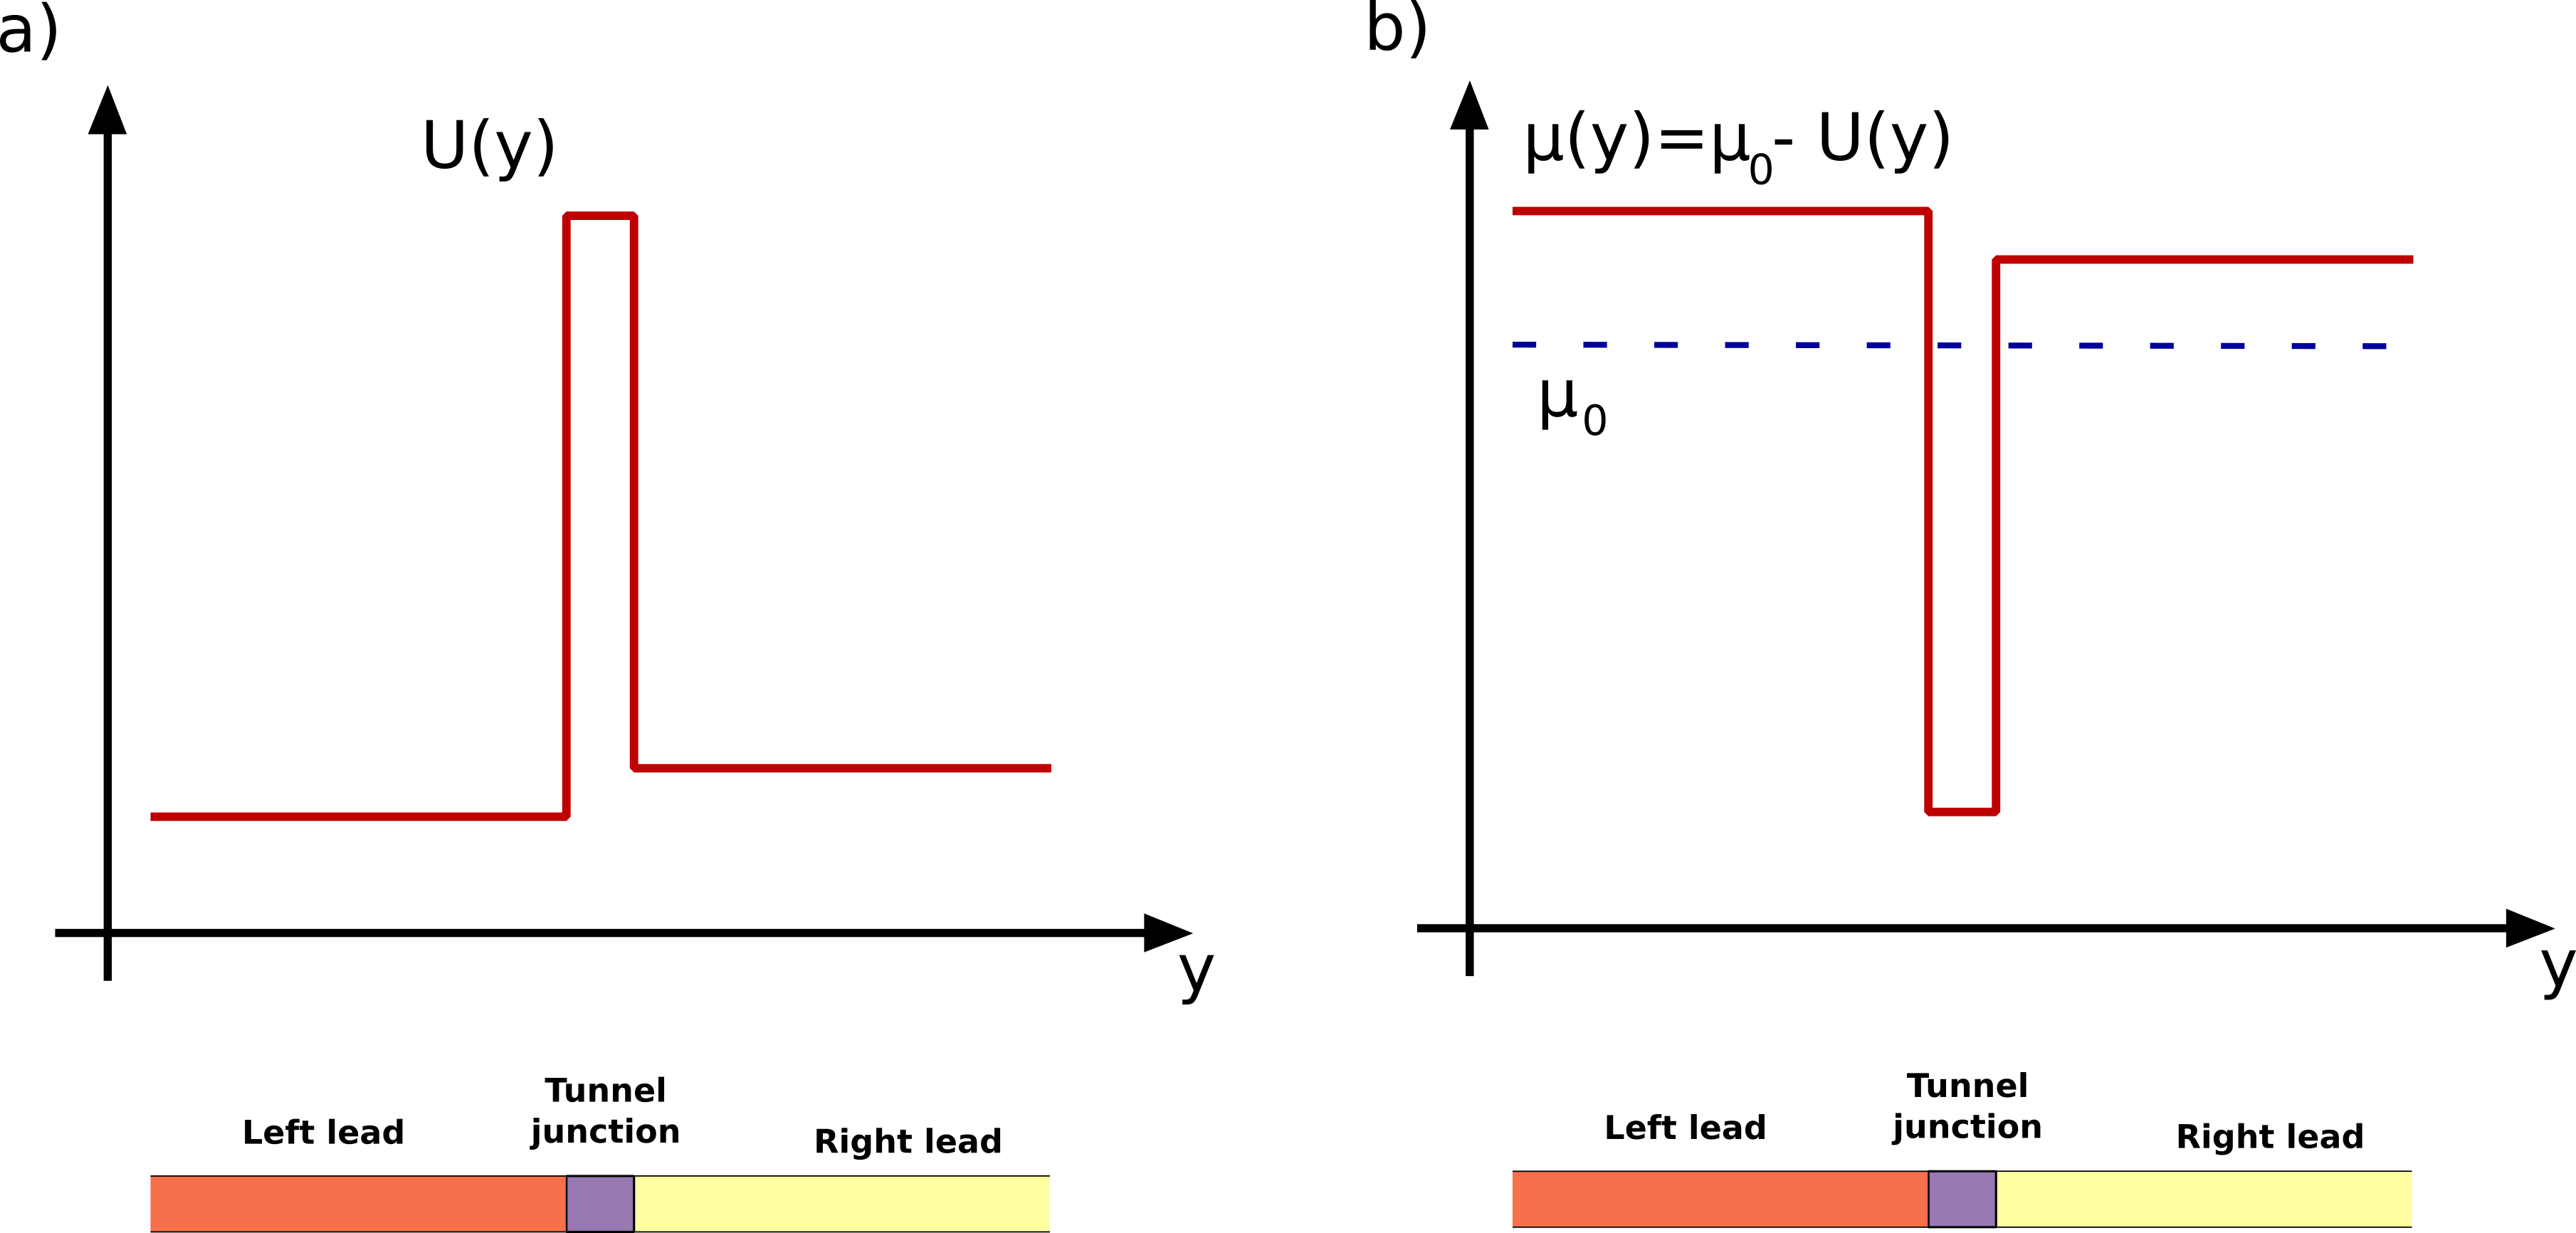
\includegraphics[width=0.8\linewidth]{images/chem_and_ext_potentials}
	\caption{(a) y-profile of external electrical field.  (b) y-profile of effective chemical potential}
	\label{fig:chemandextpotentials}
\end{figure}


Finally, the BdG Hamiltonian for the model reads:

\begin{equation}
H
=
\br{
	\frac{p^2}{2m}
	-\mu\br{y}
}\tau_z
+
u p \sigma_z \tau_z
+
B\sigma_x	
+
\Delta\tau_{\phi\br{y}}
\end{equation}

with

\begin{equation}
	\mu\br{y}
	=
	\begin{cases}
		\mu_L,~~~  -\frac{L}{2}<y\\
		\mu_b,~~ -\frac{L}{2} <y <\frac{L}{2}\\
		\mu_R, ~~~~ \frac{L}{2}< y  
	\end{cases}
	~~~~~~~~
	\phi\br{y}
	=
	\begin{cases}
		\phi_L,&~~~  -\frac{L}{2}<y\\
		\phi_R
		\frac{\frac{L}{2}+y}{L}
		+
		\phi_L
		\frac{\frac{L}{2}-y}{L},
		&~~ -\frac{L}{2} <y <\frac{L}{2}\\
		\phi_R, &~~~~ \frac{L}{2}< y 
	\end{cases}
\end{equation}
and the $ L $ being the size of the junction. Note, that the parameters $ B $, $ u $, $ \Delta $ and $ m $ are taken to be unique within all the system.
 
  This setting is close to the one of the models  considered by Oreg et al. in \cite{Oreg_2010} ("\textit{Spatially varying $ \mu $}" section). The difference is in a profile of $ \mu\br{y} $ -- Oreg et al.  introduced a step in effective chemical potential, while here this function possesses a well.  
  
It can be argued, that superconducting correlations are not possible in thin wires due to the presence of fluctuations. However in real systems this difficulty can be avoided with the help of the proximity effect. The wire itself is assumed to be metallic or semiconductor, and being put close to a strong superconductor. Due to proximity effect it's possible to obtain a presence of order parameter inside initially nonsuperconducting wire.